\documentclass[12pt]{article}

\usepackage{geometry}
\geometry{a4paper, left=1in, right=1in, top=1in, bottom=1in}
\usepackage{amsmath}
\usepackage{amsmath,amsfonts,amssymb}
\usepackage{graphicx}
\usepackage{enumitem}
\usepackage{titlesec}
\usepackage{fancyhdr}
\usepackage{hyperref}
\usepackage{floatrow}
\usepackage{geometry}
\usepackage{fancyhdr}
\usepackage{empheq}
\usepackage[svgnames]{xcolor}
\usepackage{xpatch}
\usepackage{subcaption} 
\makeatletter
\newcommand{\colorboxed}[1]{\fcolorbox{Black}{White}{\m@th$\displaystyle#1$}}
\xpatchcmd{\@Aboxed}{\boxed}{\colorboxed}{}{}
\makeatother

\title{{\bf CS663 Assignment 2}}
\author{Saksham Rathi, Kavya Gupta, Shravan Srinivasa Raghavan}
\date{September 2024}
\begin{document}
\maketitle
\clearpage
\tableofcontents
\clearpage
\section*{Question 8}
\addcontentsline{toc}{section}{Question 8}
    The results of doing local and global histogram equalisation is as follows:
    
    \begin{figure}[h!]
        \centering
        
        % First row of images (3 images)
        \begin{subfigure}[b]{0.3\textwidth}
            \centering
            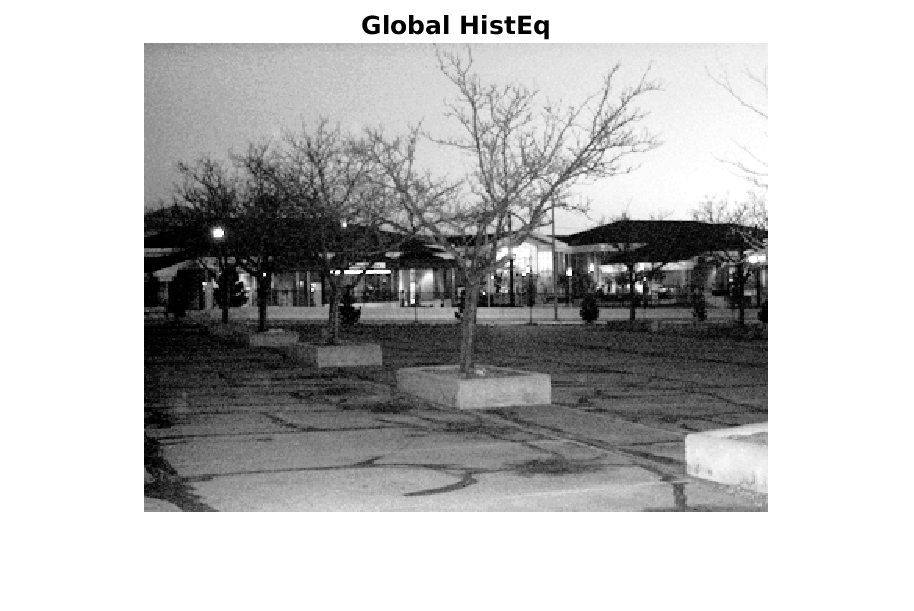
\includegraphics[width=\textwidth]{../images/LC1_globalHistEq.png}
            \caption{Global HistEq}
        \end{subfigure}
        \hfill
        \begin{subfigure}[b]{0.3\textwidth}
            \centering
            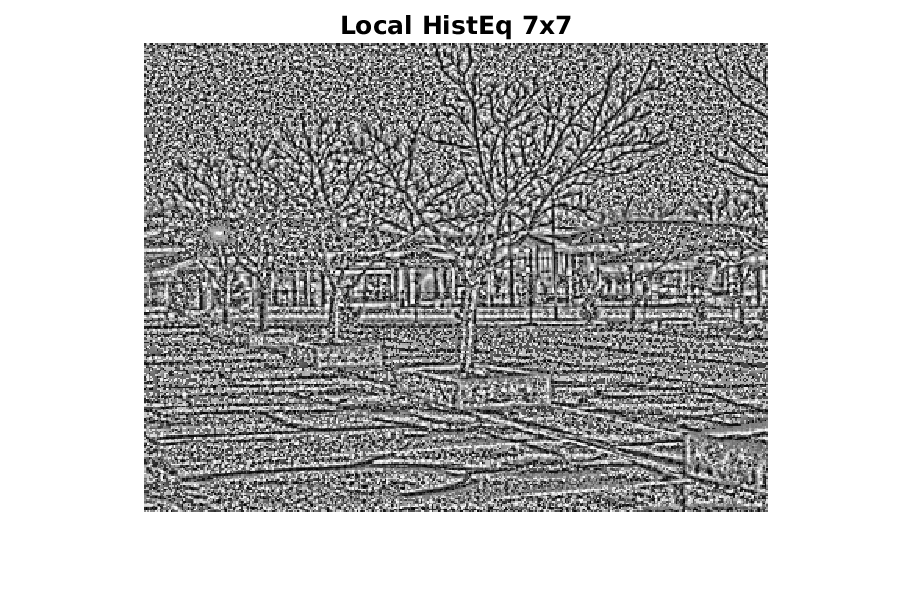
\includegraphics[width=\textwidth]{../images/LC1_localHistEq_7x7.png}
            \caption{Local HistEq 7x7}
        \end{subfigure}
        \hfill
        \begin{subfigure}[b]{0.3\textwidth}
            \centering
            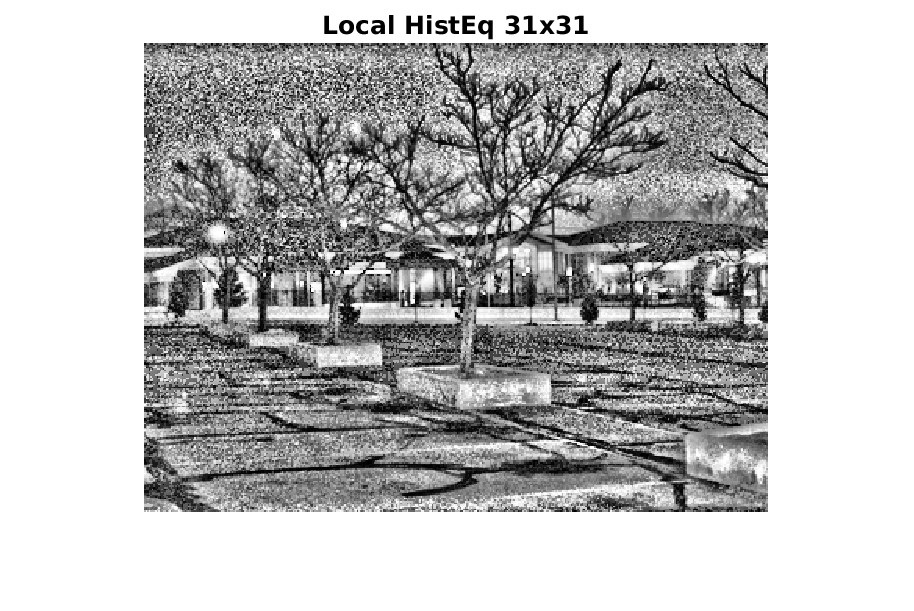
\includegraphics[width=\textwidth]{../images/LC1_localHistEq_31x31.png}
            \caption{Local HistEq 31x31}
        \end{subfigure}
        
        \vspace{10pt} % Space between the two rows
        
        % Second row of images (3 images)
        \begin{subfigure}[b]{0.3\textwidth}
            \centering
            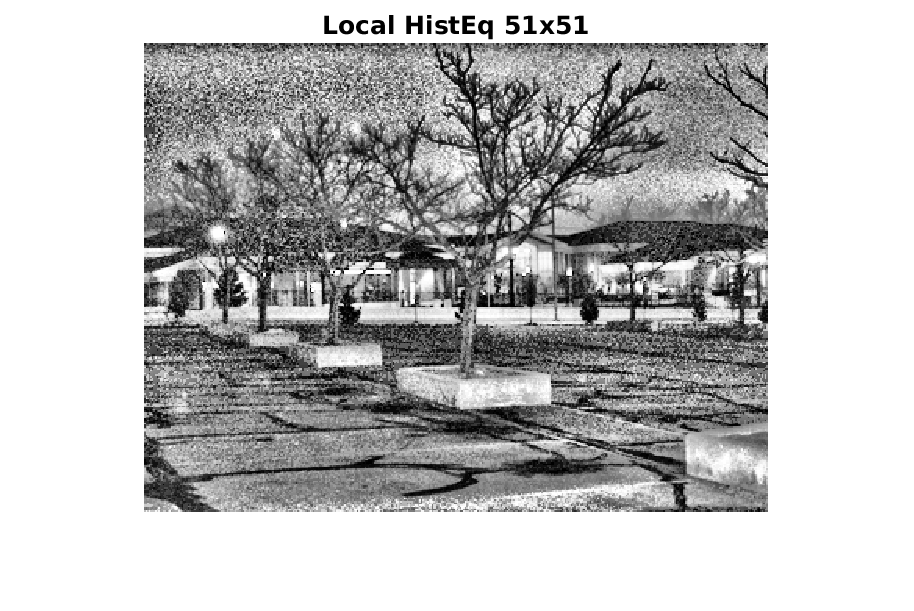
\includegraphics[width=\textwidth]{../images/LC1_localHistEq_51x51.png}
            \caption{Local HistEq 51x51}
        \end{subfigure}
        \hfill
        \begin{subfigure}[b]{0.3\textwidth}
            \centering
            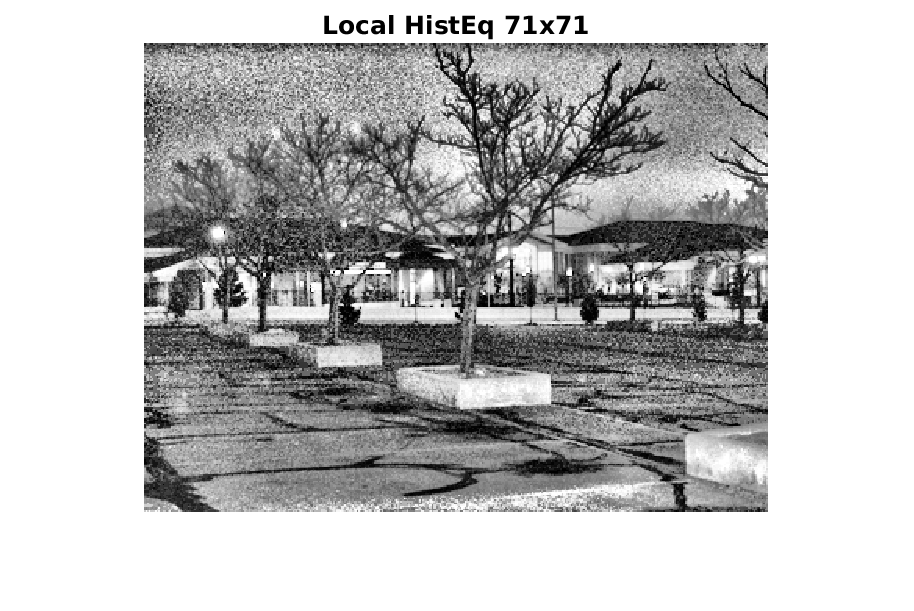
\includegraphics[width=\textwidth]{../images/LC1_localHistEq_71x71.png}
            \caption{Local HistEq 71x71}
        \end{subfigure}
        \hfill
        \begin{subfigure}[b]{0.3\textwidth}
            \centering
            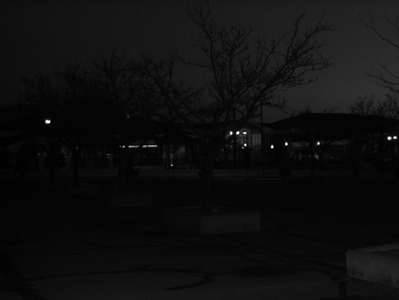
\includegraphics[width=\textwidth]{../images/LC1.png}
            \caption{Original LC1}
        \end{subfigure}
    
        \caption{Results for LC1.png}
    \end{figure}

    \begin{figure}[h!]
        \centering
        
        % First row of images (3 images)
        \begin{subfigure}[b]{0.3\textwidth}
            \centering
            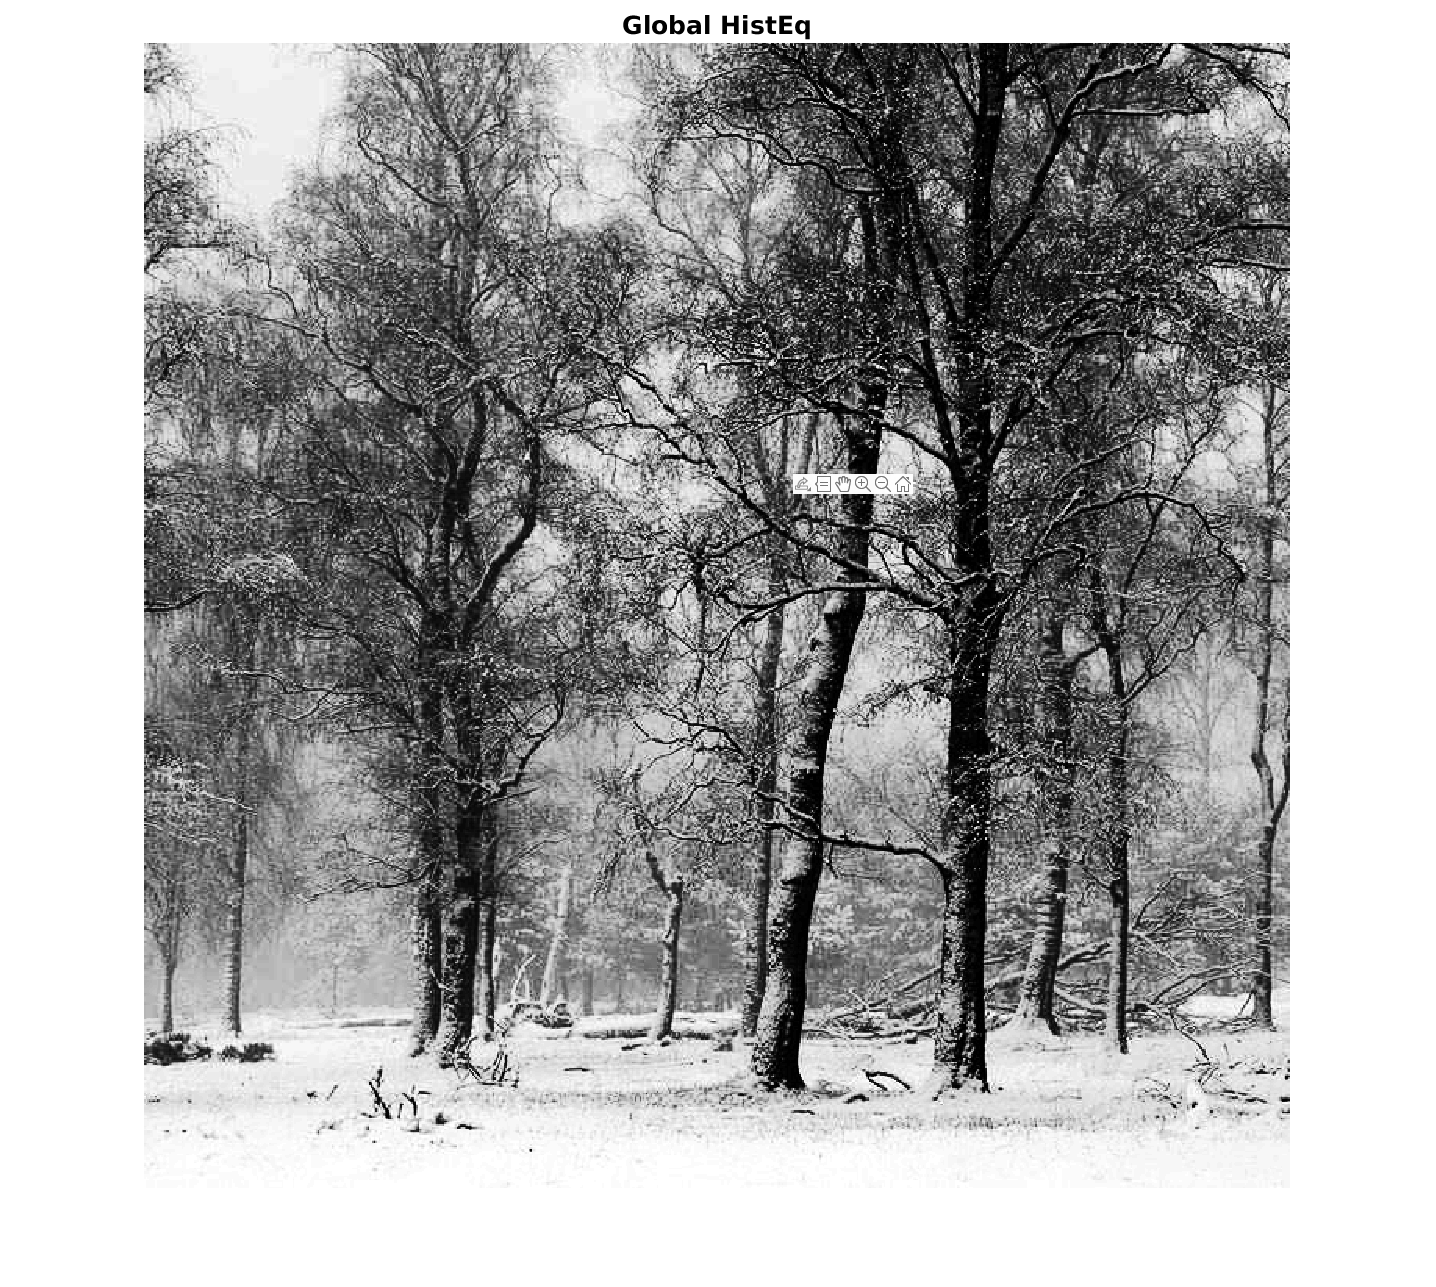
\includegraphics[width=\textwidth]{../images/LC2_globalHistEq.png}
            \caption{Global HistEq}
        \end{subfigure}
        \hfill
        \begin{subfigure}[b]{0.3\textwidth}
            \centering
            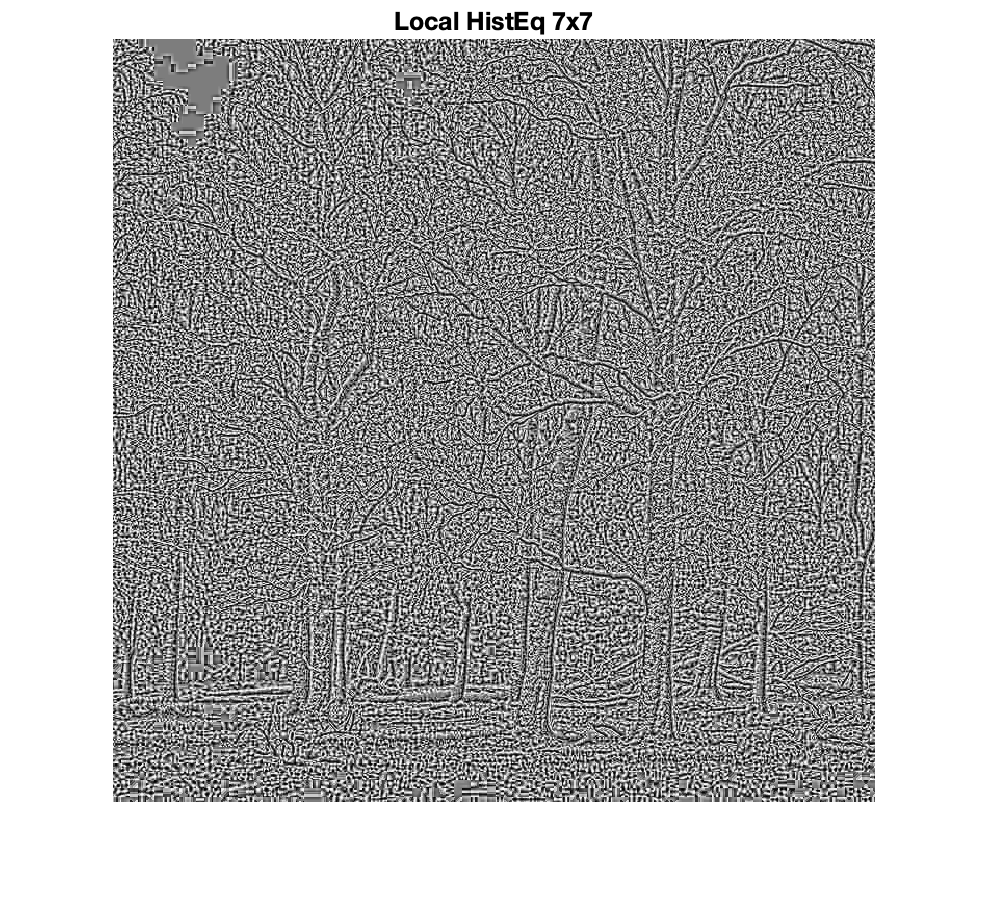
\includegraphics[width=\textwidth]{../images/LC2_localHistEq_7x7.png}
            \caption{Local HistEq 7x7}
        \end{subfigure}
        \hfill
        \begin{subfigure}[b]{0.3\textwidth}
            \centering
            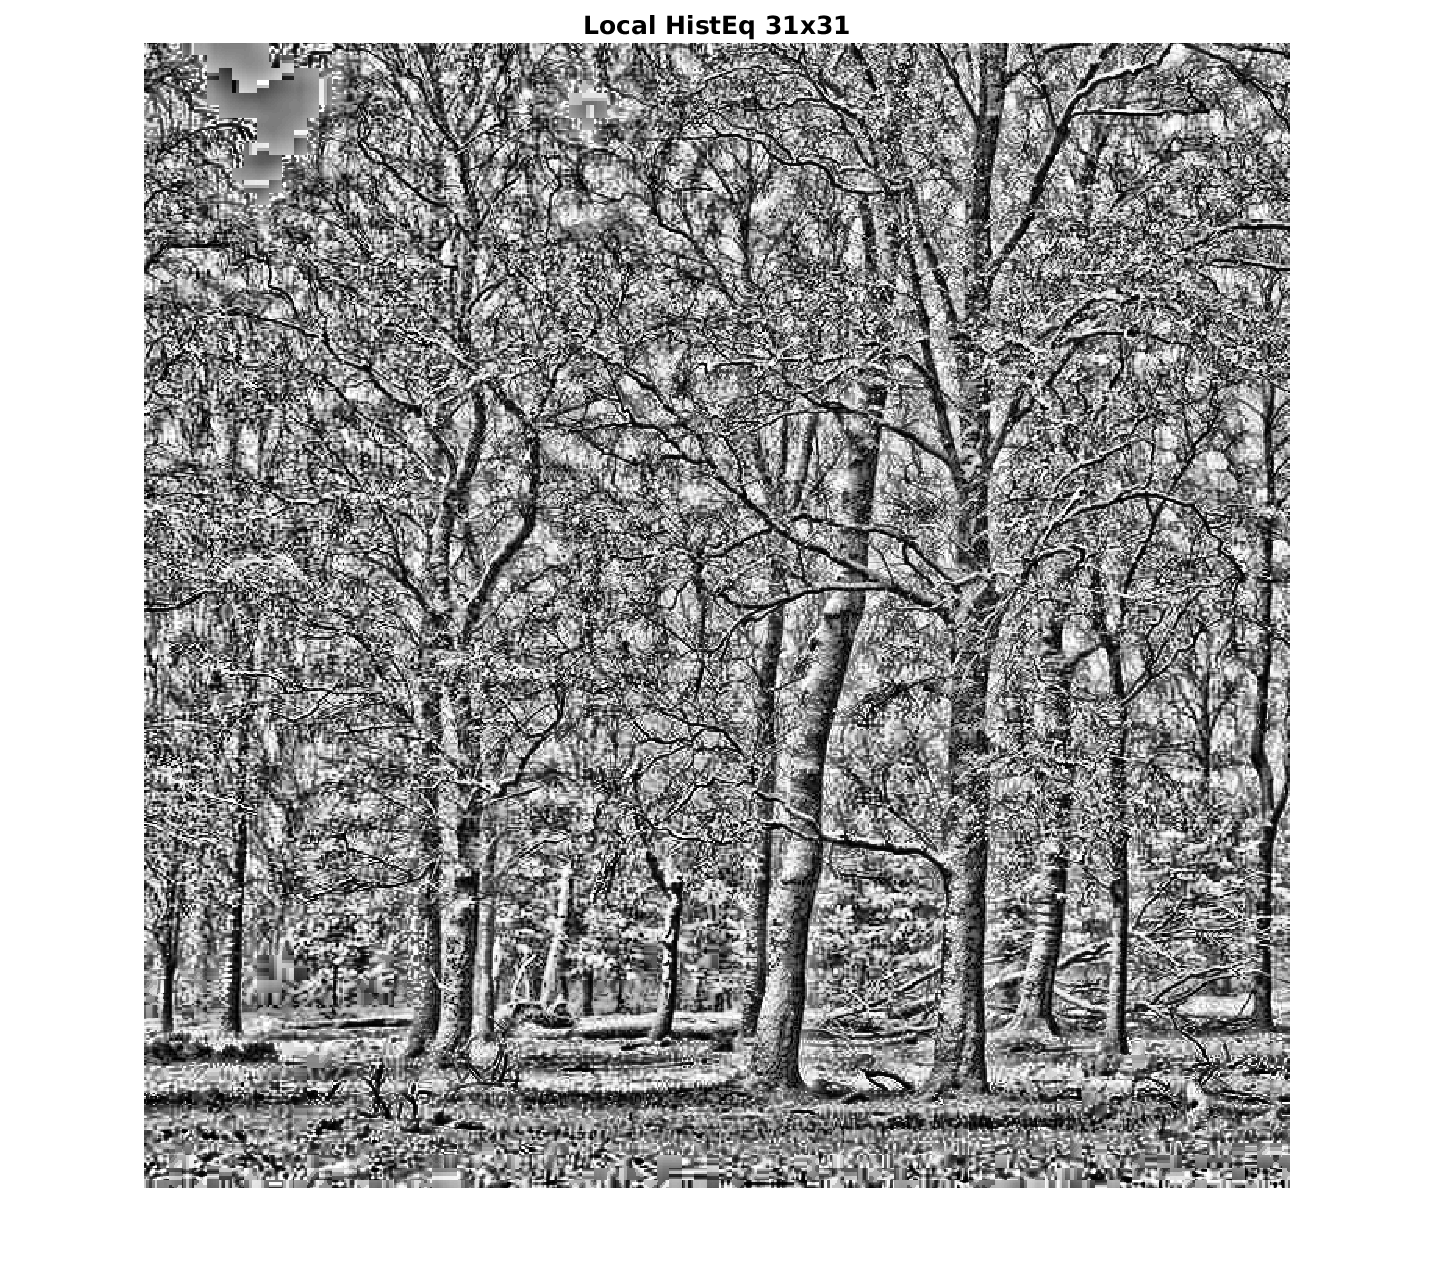
\includegraphics[width=\textwidth]{../images/LC2_localHistEq_31x31.png}
            \caption{Local HistEq 31x31}
        \end{subfigure}
        
        \vspace{10pt} % Space between the two rows
        
        % Second row of images (3 images)
        \begin{subfigure}[b]{0.3\textwidth}
            \centering
            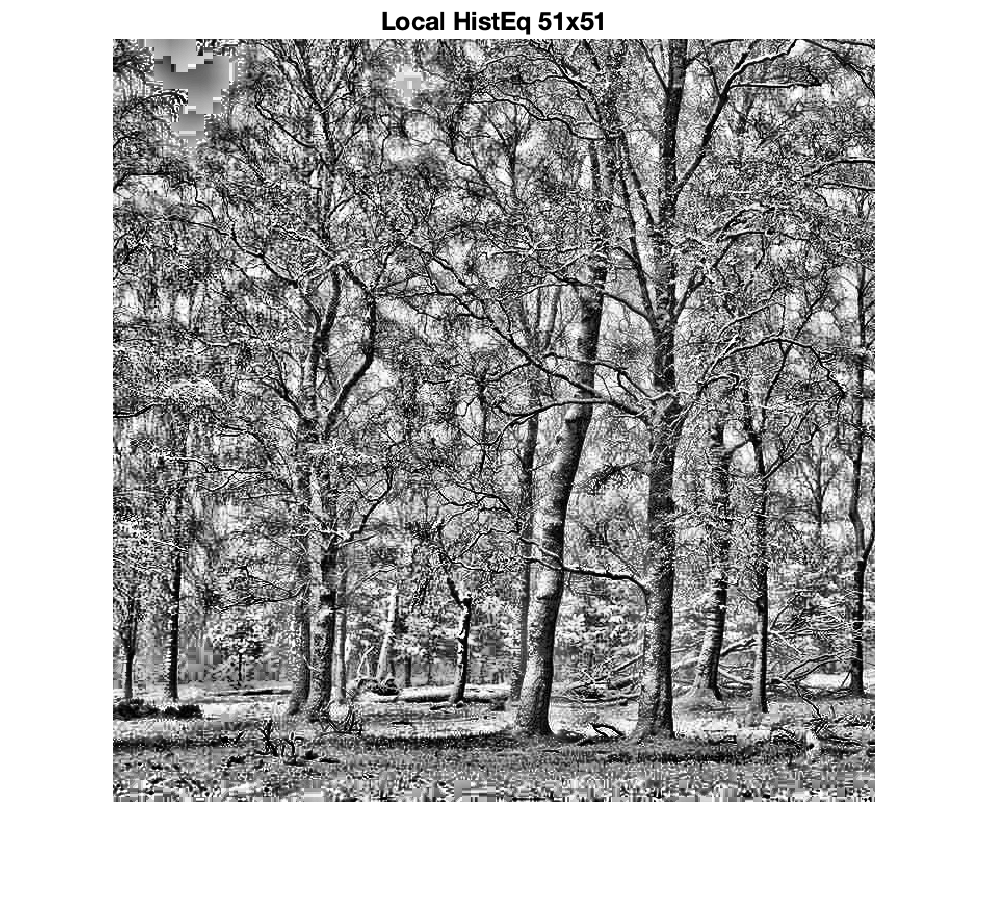
\includegraphics[width=\textwidth]{../images/LC2_localHistEq_51x51.png}
            \caption{Local HistEq 51x51}
        \end{subfigure}
        \hfill
        \begin{subfigure}[b]{0.3\textwidth}
            \centering
            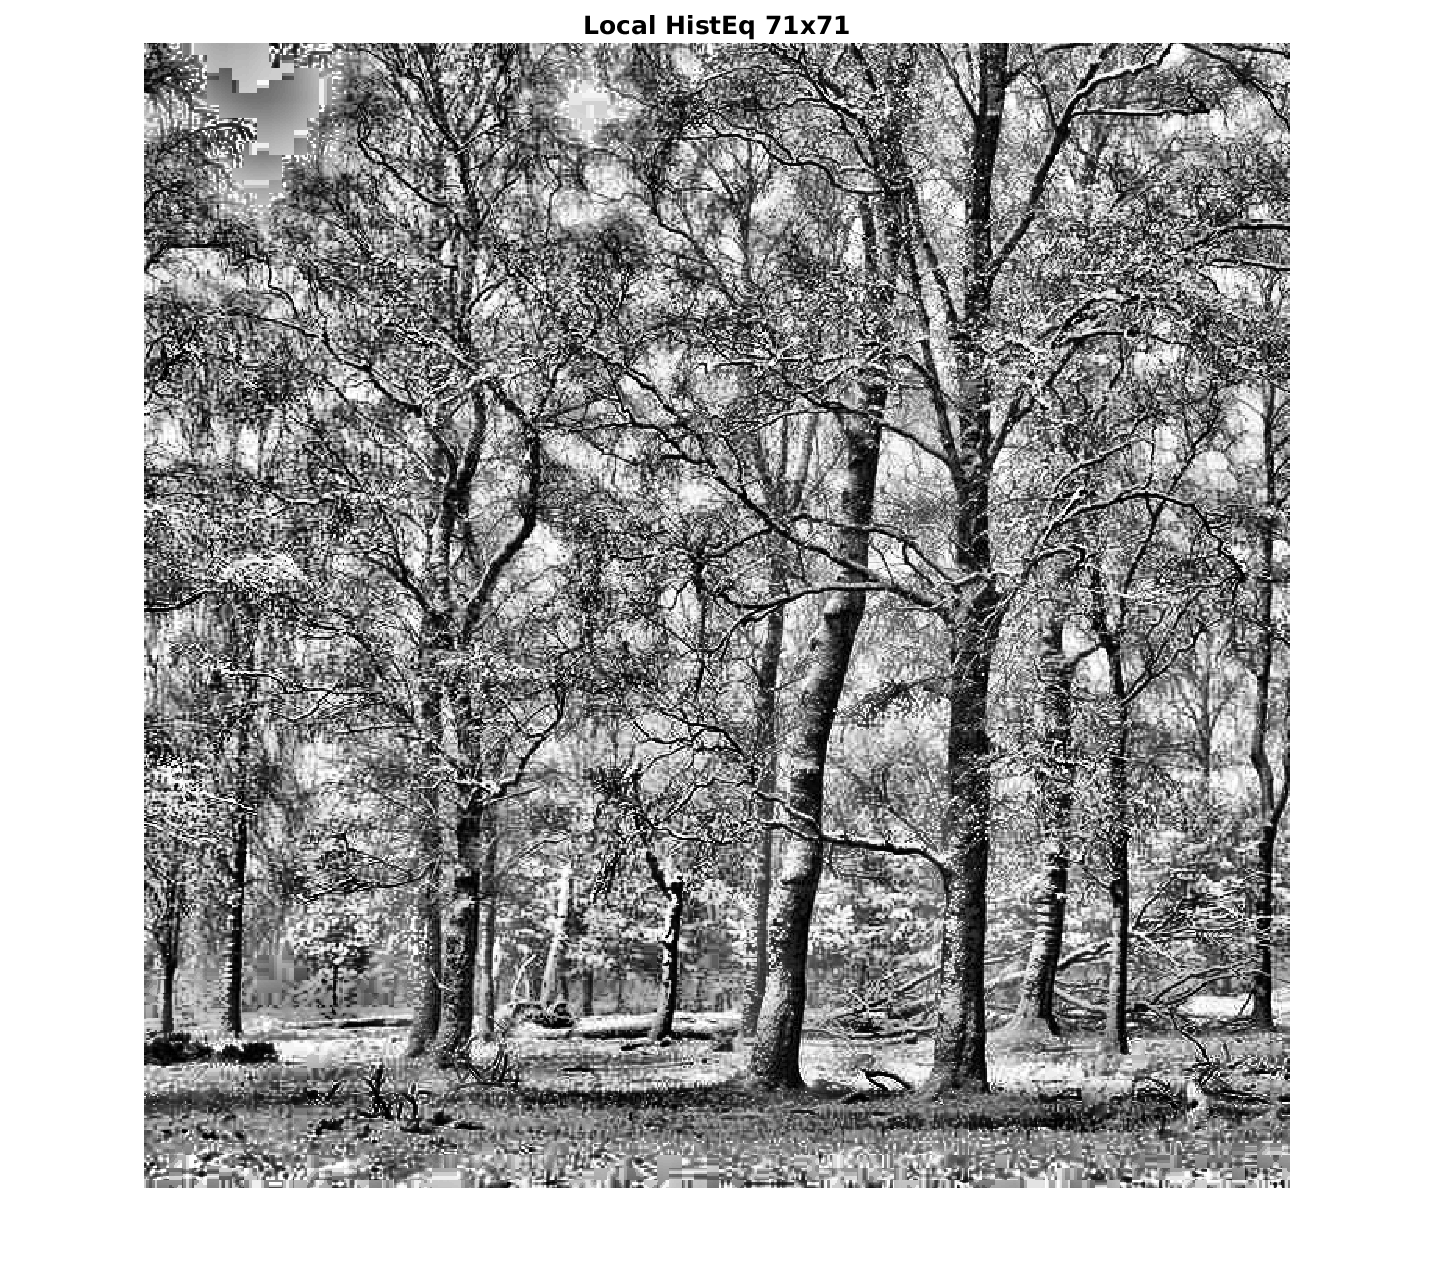
\includegraphics[width=\textwidth]{../images/LC2_localHistEq_71x71.png}
            \caption{Local HistEq 71x71}
        \end{subfigure}
        \hfill
        \begin{subfigure}[b]{0.3\textwidth}
            \centering
            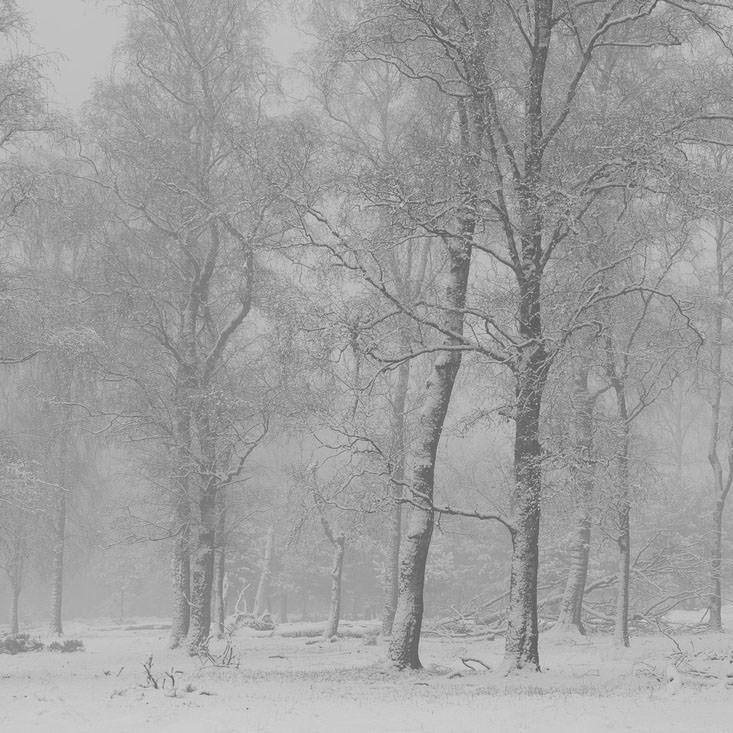
\includegraphics[width=\textwidth]{../images/LC2.jpg}
            \caption{Original LC2}
        \end{subfigure}
    
        \caption{Results for LC2.png}
    \end{figure}

    Upon comparing the global and local histogram equalisation for LC1 the patches outlined in the red boxes
    were found to have \textbf{better contrast} in the local method than in the global method:

    \begin{figure}[ht]
        \centering
        
        % First row of images (3 images)
        \begin{subfigure}[b]{0.4\textwidth}
            \centering
            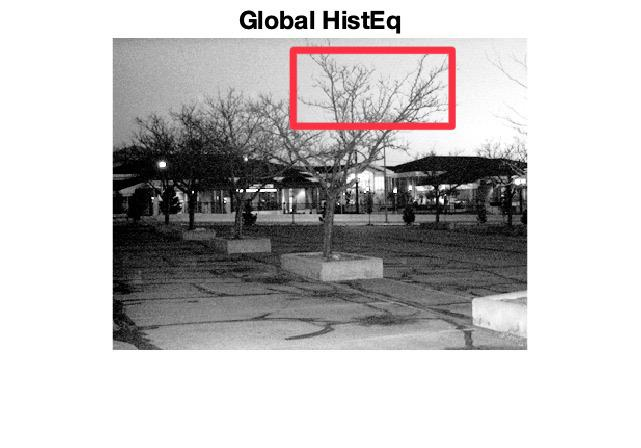
\includegraphics[width=\textwidth]{../images/LC1_globalHistEq_1.jpeg}
            \caption{Global HistEq}
        \end{subfigure}
        \hfill
        \begin{subfigure}[b]{0.4\textwidth}
            \centering
            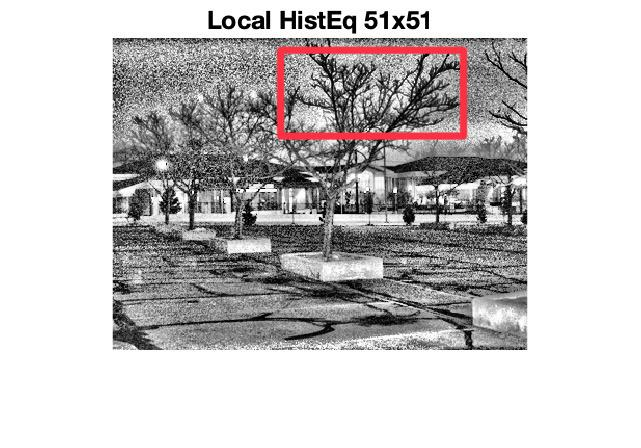
\includegraphics[width=\textwidth]{../images/LC1_localHistEq_1.jpeg}
            \caption{Local HistEq}
        \end{subfigure}
        
        \vspace{10pt} % Space between the two rows
        
        % Second row of images (3 images)
        \begin{subfigure}[b]{0.4\textwidth}
            \centering
            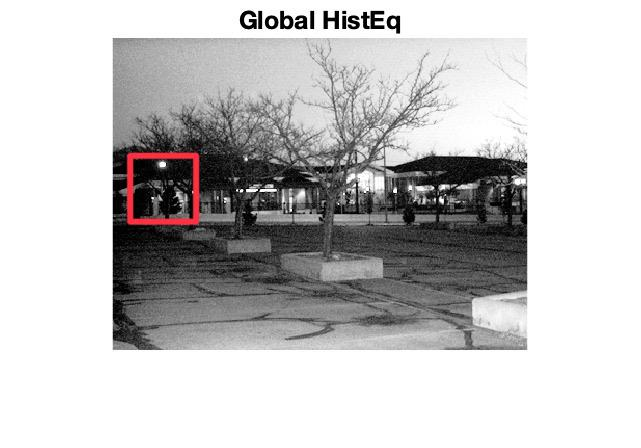
\includegraphics[width=\textwidth]{../images/LC1_globalHistEq_2.jpeg}
            \caption{Global HistEq}
        \end{subfigure}
        \hfill
        \begin{subfigure}[b]{0.4\textwidth}
            \centering
            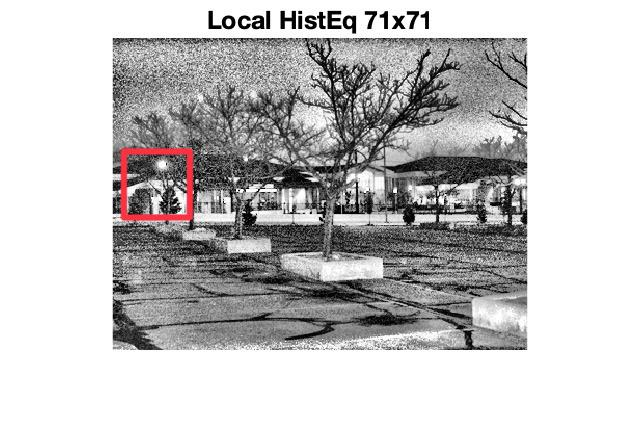
\includegraphics[width=\textwidth]{../images/LC1_localHistEq_2.jpeg}
            \caption{Local HistEq}
        \end{subfigure}
    
        \caption{Contrasts for LC1.png}
    \end{figure}

    Similar results were obtained for the image LC2:

    \begin{figure}[ht]
        \centering
        
        % First row of images (3 images)
        \begin{subfigure}[b]{0.4\textwidth}
            \centering
            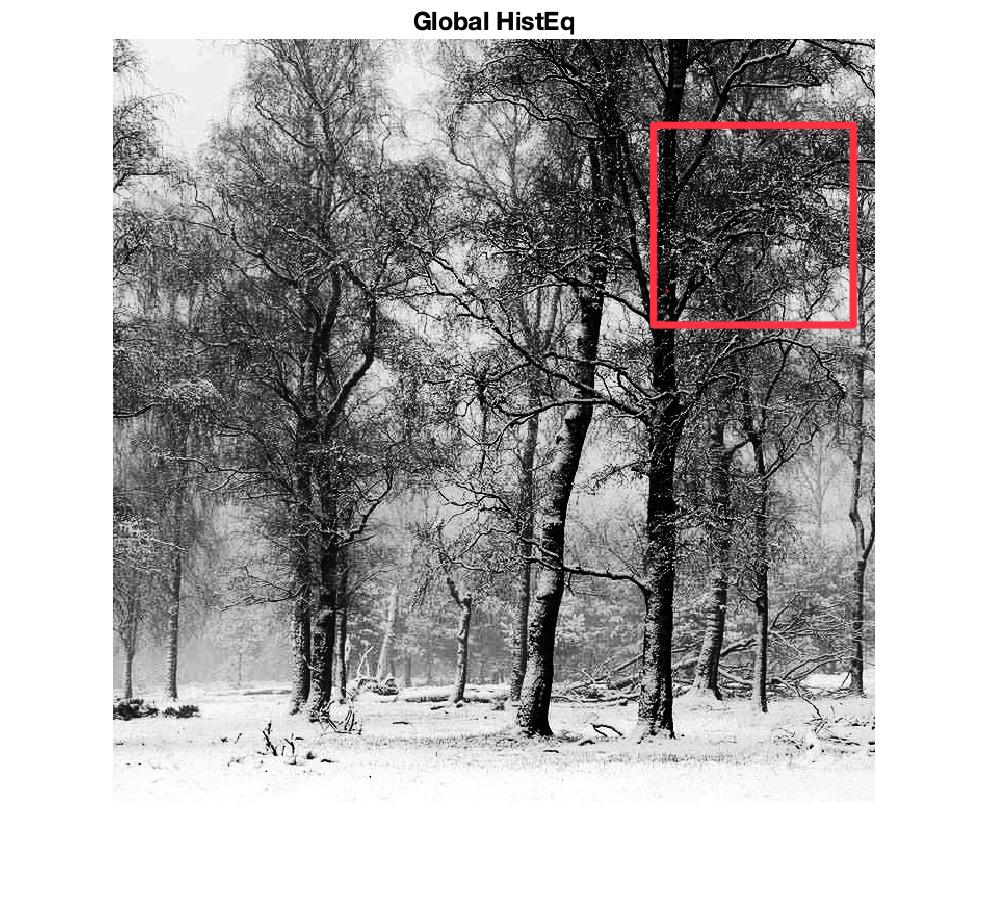
\includegraphics[width=\textwidth]{../images/LC2_globalHistEq_1.jpeg}
            \caption{Global HistEq}
        \end{subfigure}
        \hfill
        \begin{subfigure}[b]{0.4\textwidth}
            \centering
            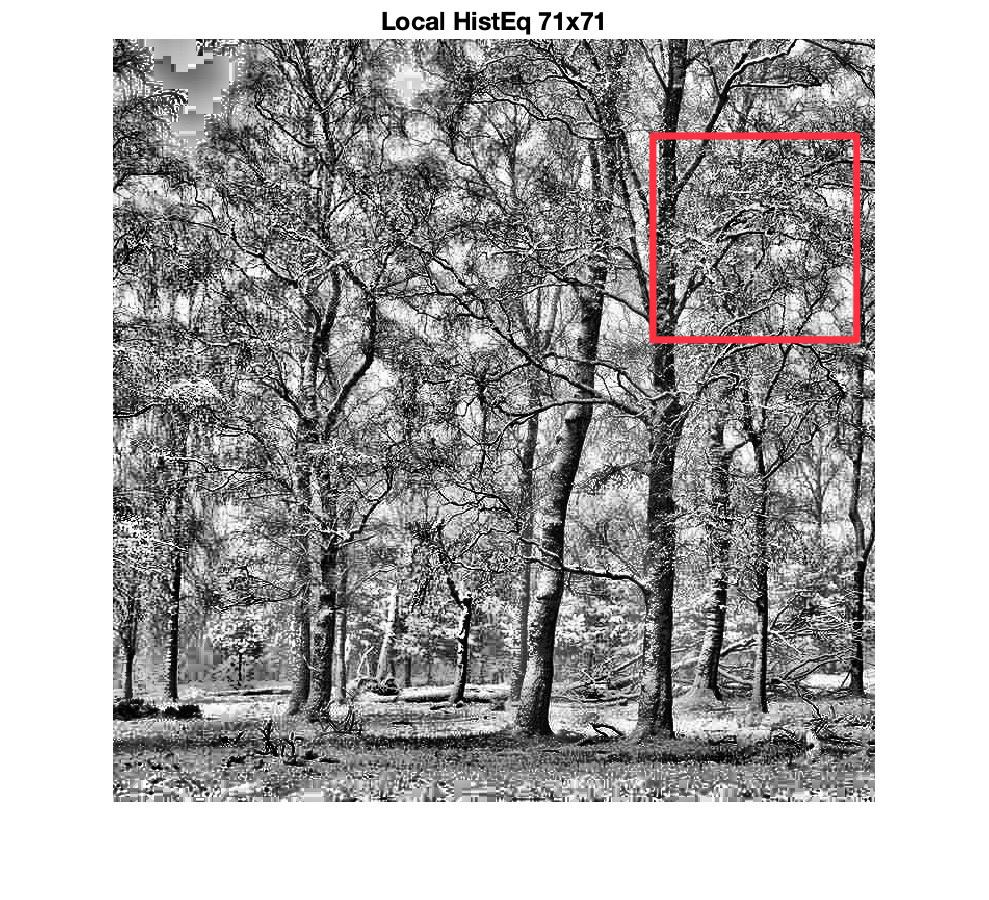
\includegraphics[width=\textwidth]{../images/LC2_localHistEq_1.jpeg}
            \caption{Local HistEq 7x7}
        \end{subfigure}
        
        \vspace{10pt} % Space between the two rows
        
        % Second row of images (3 images)
        \begin{subfigure}[b]{0.4\textwidth}
            \centering
            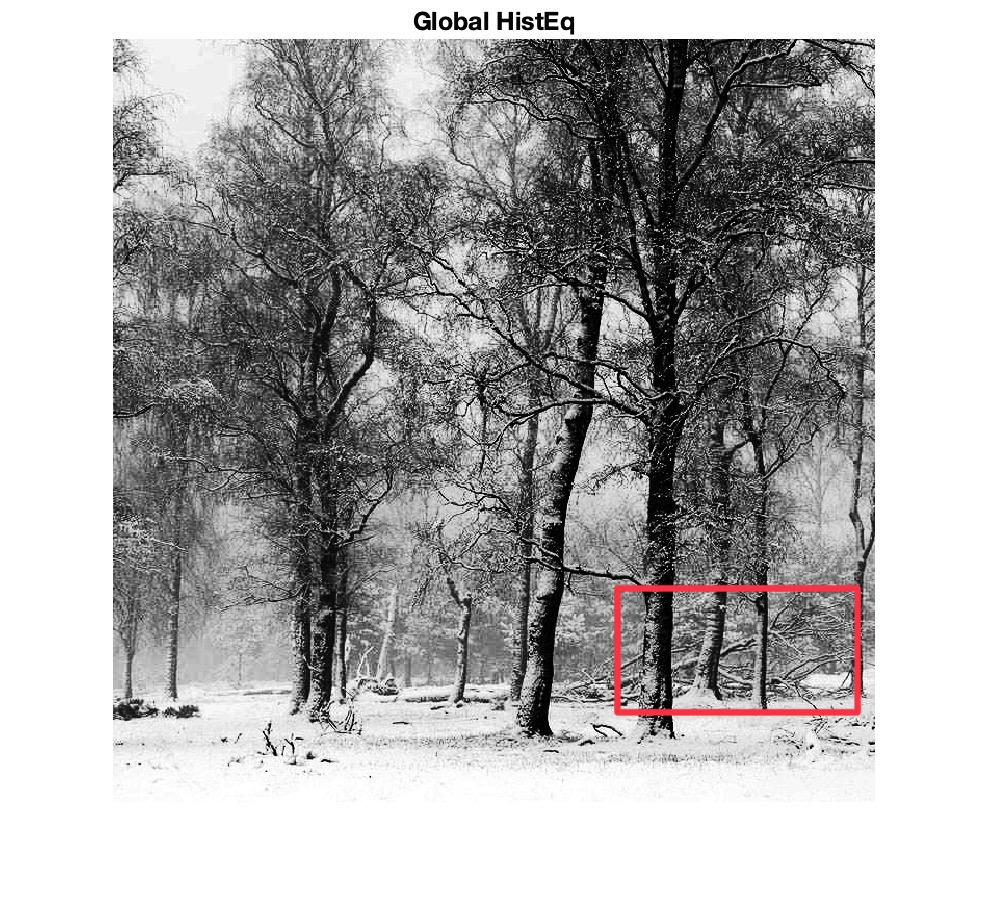
\includegraphics[width=\textwidth]{../images/LC2_globalHistEq_2.jpeg}
            \caption{Global Histeq}
        \end{subfigure}
        \hfill
        \begin{subfigure}[b]{0.4\textwidth}
            \centering
            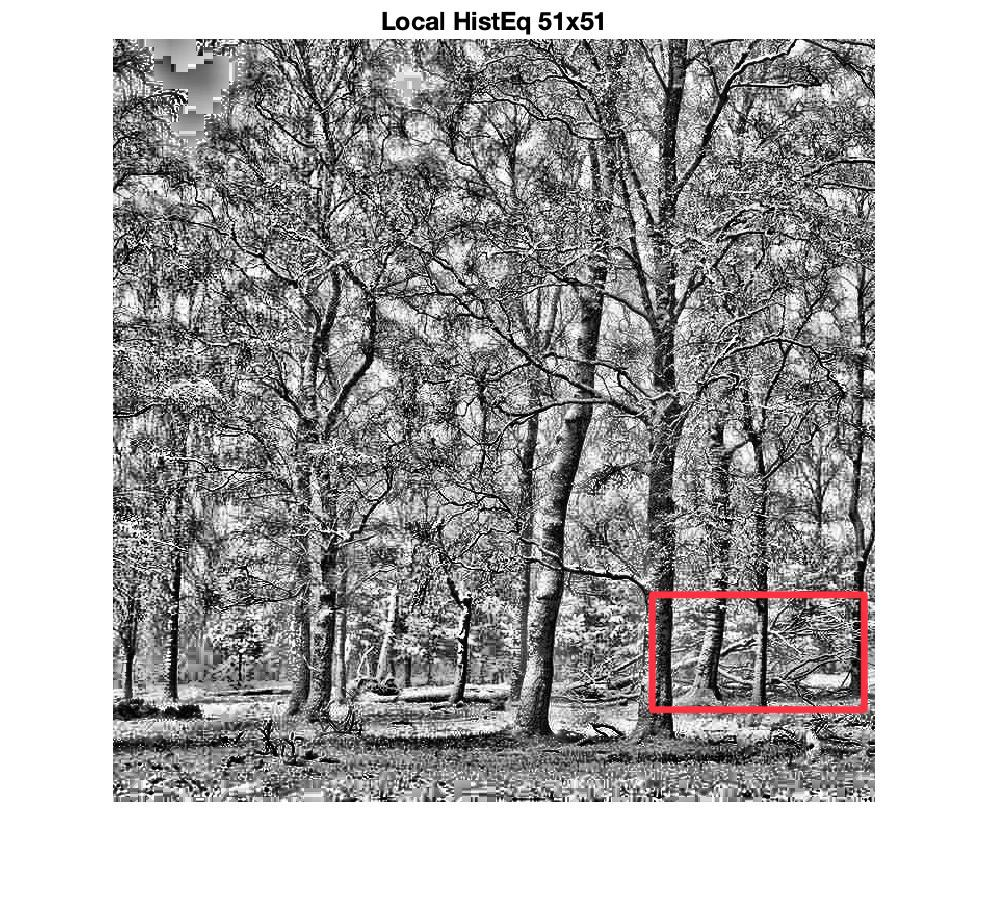
\includegraphics[width=\textwidth]{../images/LC2_localHistEq_2.jpeg}
            \caption{Local HistEq 71x71}
        \end{subfigure}
    
        \caption{Contrasts for LC2.jpg}
    \end{figure}

    \subsection*{Explanation}
    Histogram equalisation uses all the pixels that are available to get better contrast. If only a small window were
    used as in the case of $7 \times 7$ local histogram method, the data is too less and the contrast is poor. So going 
    by this argument, we must be getting the best results from using the entire image. This is not so because some regions
    of the image have nothing to do with the other and have no influence on the intensities of each other's pixels. Finding 
    a big enough window for local histogram equalisation gives the best results. On average the $51 \times 51$ and 
    $71 \times 71$ windows seem to work better than the global method.
    \begin{enumerate}
        \item For LC1, the regions where the buildings are shadowed by trees is contrasted very well in the local method. 
        \item For LC2, the branches at the top of tall trees and the logs on the ground are well contrasted in the local method.
    \end{enumerate}
    In both cases we are looking at the windows of sizes $51 \times 51$ and $71 \times 71$.
\end{document}